% This is samplepaper.tex, a sample chapter demonstrating the
% LLNCS macro package for Springer Computer Science proceedings;
% Version 2.21 of 2022/01/12
%
\documentclass[runningheads]{llncs}
%
\usepackage[T1]{fontenc}
\usepackage{graphicx}
\usepackage{amsmath}
\usepackage{amsfonts}
\usepackage{color}
% \renewcommand\UrlFont{\color{blue}\rmfamily}


\begin{document}

\title{Particle Filter and Support Vector Regression: Individual and collective performance}
%
%\titlerunning{Abbreviated paper title}
% If the paper title is too long for the running head, you can set
% an abbreviated paper title here
%
\author{First Author\inst{1}\orcidID{0000-1111-2222-3333} \and
Second Author\inst{2,3}\orcidID{1111-2222-3333-4444} \and
Third Author\inst{3}\orcidID{2222--3333-4444-5555}}
%
\authorrunning{F. Author et al.}
% First names are abbreviated in the running head.
% If there are more than two authors, 'et al.' is used.
%
\institute{Princeton University, Princeton NJ 08544, USA \and
Springer Heidelberg, Tiergartenstr. 17, 69121 Heidelberg, Germany
\email{lncs@springer.com}\\
\url{http://www.springer.com/gp/computer-science/lncs} \and
ABC Institute, Rupert-Karls-University Heidelberg, Heidelberg, Germany\\
\email{\{abc,lncs\}@uni-heidelberg.de}}
%
\maketitle              % typeset the header of the contribution
%
\begin{abstract}
The abstract should briefly summarize the contents of the paper in
150--250 words.

\keywords{First keyword  \and Second keyword \and Another keyword.}
\end{abstract}
%
%
%

\section{Introduction}
\label{sec:intro}
Los algoritmos Sequential Monte Carlo (SMC) son técnicas utilizados para simular muestras en forma secuencial a partir de distribuciones que evolucionan en el tiempo, se caracterizan por ser altamente flexibles y de extensa aplicabilidad en muchos campos de la ciencia.
 En particular, los filtros de partículas (PF) es un algoritmo SMC. Los PF fueron desarrollados en la década de los $(1990)$, por  Gordon et. al $(1993)$, Kitagawa $(1996)$, Del Moral $(1996)$, Doucet et. al $(2000)$, Doucet et. al $(2001)$, Godsill et. al $(2000)$, Ristic et. al $(2003)$, entre otros, con el propósito de aproximar distribuciones arbitrarias, posiblemente 
 multimodales y en espacios de alta dimensiones. El método consiste en generar un conjunto de muestras pesadas llamadas partículas y una
 distribución prior para aproximar la densidad a posterior de los estados desconocidos. El paso de predicción supone una recursión Markoviana que se actualiza en forma iterativa  sobre la base de los estados 
 predichos en tiempos pasados.\\
%SVR PF
Lo mas simple es promediar ambas predicciones y ver los resultados.

Usar SVR para predecir el valor y hacer correcciones con PF. Mover las particulas dependiendo de las predicciones de SVR

Usar SVR dentro de la funcion de movimiento de las particulas. Puede ser predecir la tasa de cambio del siguiente paso y que las particulas se muevan segun ese valor.




\begin{table}
\caption{Table captions should be placed above the
tables.}\label{tab1}
\begin{tabular}{|l|l|l|}
\hline
Heading level &  Example & Font size and style\\
\hline
Title (centered) &  {\Large\bfseries Lecture Notes} & 14 point, bold\\
1st-level heading &  {\large\bfseries 1 Introduction} & 12 point, bold\\
2nd-level heading & {\bfseries 2.1 Printing Area} & 10 point, bold\\
3rd-level heading & {\bfseries Run-in Heading in Bold.} Text follows & 10 point, bold\\
4th-level heading & {\itshape Lowest Level Heading.} Text follows & 10 point, italic\\
\hline
\end{tabular}
\end{table}


\begin{figure}
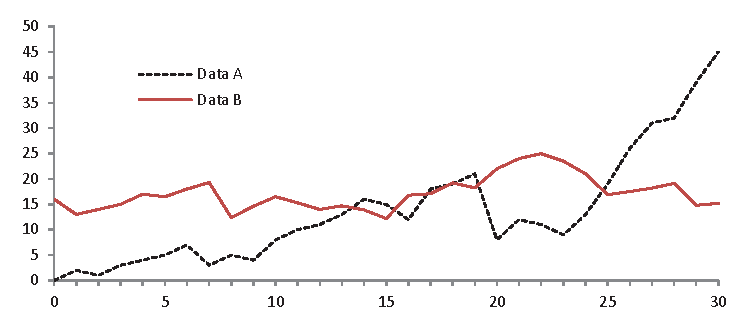
\includegraphics[width=\textwidth]{fig1.eps}
\caption{A figure caption is always placed below the illustration.
Please note that short captions are centered, while long ones are
justified by the macro package automatically.} \label{fig1}
\end{figure}

The remaining of this paper is structured as follows: Section \ref{sec:related_work} extend the background of this work and explains similar works to the one proposed in this study. Section \ref{sec:material_method} describes the metrics, data sets and overviews the proposed approach used in this study. Section \ref{sec:results} gathers the main results obtained from the experiments. Section \ref{sec:disscussion} explores the significance of the work's results. Finally, the concluding remarks are drawn in Section \ref{sec:conclusions}. 



%%%%%%%%%%%%%%%%%%%%%%%%%%%%%%%%%%%%%%%%%%%%%%%%%%%%%%%%%%%%%%%%%%%%%%%%%%%%%%%%%%%%%%%%%%
\section{Related Work}
\label{sec:related_work}
SABA

\section{Materials and Methods}
\label{sec:material_methods}

\subsection{SARIMA}
%El pronóstico de series temporales es un área de investigación importante
%en el aprendizaje automático, debido a la consideración de la información del pasado
%para predecir el futuro.
Time series forecasting is an important research area in machine learning, due to the 
consideration of information from the past to predict the future.
Proper forecasting has significant value in
many areas of science such as: economics, meteorology, agriculture, biology,
 physics and health among many others.
 When the time series is not stationary, it can be decomposed into 
 deterministic and stochastic components to obtain better prediction performance.
% El pronostico oportuno tiene un valor significativo en
%muchas áreas de las ciencias tales como en: economía, meteorología, agricultura,
%biología, física y salud entre muchas otras.
%Cuando la serie de tiempo no es estacionaria se puede descomponer en componentes
%deterministico y estocásticos para obtener mejor desempeño de predicción.
%Las características de la tendencia y estacionalidad son tratados
%por  el  modelo de promedio móvil integrado autorregresivo (ARIMA$(p,d,q)$)
The characteristics of the trend and seasonality are treated
by the autoregressive integrated moving average model (ARIMA$(p,d,q)$)
where $p$ is the number of auto regressive terms, $d$ is the
order of differencing, $q$ is the number of moving average terms.
%El ARIMA es uno de los modelos de pronostico más utilizado  por su flexibilidad.
%Sin embargo, tiene algunas limitaciones  por la suposición
%de la linealidad entre el valor presente y el valor pasado, y el ruido
%aleatorio en el modelo; se considera  la suposición de tendencia aditiva 
%pero no toma en cuenta los episodios estacionales, para mayores detalle ver
ARIMA is one of the most widely used forecast models due to its flexibility. 
However, it has some limitations due to the assumption of linearity between 
the present value and the past value, and random noise in the model; 
the assumption of additive tendency is considered but it does not take
 into account the seasonal episodes, for more details see
K Abdul Hamid,  et., al. $(2023)$, Aisyah et., al. $(2021)$, 
Dama and Sinoquet $(2021)$ 
y sus referencias entre otros.\\
A time series $\{X_{t}\}$ follows an ARIMA$(p,d,q)$ process if:
\begin{align*}
 \Phi_{p}(L)\left(1-L\right)^{d}X_{t}= \Theta_{q}(L)\epsilon_{t}
\end{align*}
where $\{\epsilon_{t}\}$ is a white noise series, $p$, $d$, $q$ are integers,
 $L$ is the backward shift operator $LX_{t}= X_{t-1}$, $L^{k}X_{t}= X_{t-k}$,
 $\Phi_{p}$ and $\Theta_{q}$ are polynomials in $L$, of orders $p$ and $q$, 
 respectively:
 \begin{align*}
 &\Phi_{p}=1-\phi_{1}L-\phi_{2}L^{2}-\ldots-\phi_{p}L^{p}\\
  &\Theta_{q}(L)=1-\alpha_{1}L-\alpha_{2}L^{2}-\ldots-\alpha_{p}L^{p}\\
\end{align*}
The best known structures of the ARIMA model are summarized in
 see Dama and Sinoquet $(2021)$:
\begin{enumerate}
\item White noise: ARIMA$(0,0,0)$,
\item Random walk process: ARIMA$(0,1,0)$,
\item Autoregression: ARIMA$(p,0,0)$,
\item Moving Avarage: ARIMA$(0,q,0)$,
\item ARMA: ARIMA$(p,0,q)$.
\end{enumerate}
Seasonal Autoregressive Integrated Moving Average Model $(SARIMA)$
 is similar to the Arima model but this model is preferable
when the time series exhibits seasonality. The SARIMA can be
expressed in terms of a composite model which can be denoted as
$(SARIMA(p; d; q)(P;D;Q)_{s})$, where  $p$, $d$ and
$q$ represent the non-seasonal AR order, no seasonal differencing,
non-seasonal MA order respectively. Also, the model parameters
$P$, $D$, $Q$ and $s$ are corresponding to the seasonal AR order,
seasonal differencing, seasonal MA order, and time span of
repeating seasonal pattern respectively. The SARIMA is not a
 linear model. A time series $\{X_{t}\}$ is generated by 
 a SARIMA process if:
 \begin{align*}
 \Phi_{p}(L)\Phi_{P}\left(L^{s}\right) (1-L)^{d}\left(1-L^{s}\right)^{D}X_{t}=\Theta_{q}(L)
 \Theta_{Q}(L^{s})\epsilon_{t}
 \end{align*}
 where $\{\epsilon_{t}\}$ is a white noise series, $p$, $d$, $q$,
  $P$, $D$, $Q$ and $s$ are integers, $L$ is the backward shift operator
 $L^{k}X_{t}= X_{t-k}$, and
  \begin{align*}
  &\Phi_{p}(L)=1-\phi_{1}L-\phi_{2}L^{2}-\ldots-\phi_{p}L^{p}\\
  &\Phi_{p}(L^{s})=1-\phi_{s}L-\phi_{2s}L^{2}-\ldots-\phi_{Ps}L^{Ps}\\
  &\Theta_{q}(L)=1-\alpha_{1}L-\alpha_{2}L^{2}-\ldots-\alpha_{p}L^{p}\\
  &\Theta_{Q}(L^{s})=1-\alpha_{s}L^{s}-\alpha_{2s}L^{2s}-\ldots-\alpha_{Qs}L^{Qs}\\
 \end{align*}
 are polynomials of degrees $p$, $P$, $q$ and $Q$, respectively, $s$ is the seasonality period, $d$ is the number of
 classical differentiations and $D$ is the number of seasonal differentiations.\\
 The best known structures of the SARIMA model are summarized in see Dama and Sinoquet $(2021)$:
 \begin{enumerate}
 	\item Seasonal ARMA: SARIMA$(0,0,0)(P,0,Q)_{s}$,
 	\item ARIMA: SARIMA$(p,d,q)(0,0,0)$,
 	\item  Additive trend-seasonality model: SARIMA$(p,d,q)(0,D,0)_{s}$.
 \end{enumerate}


\subsection{Support Vector Regression}
The Support Vector Regression (SVR) algorithm was formulated by Vapnik and Chervonenkis $(1964)$
and is a machine-learning algorithm that is perhaps the most elegant of all kernel-learning 
methods. The SVR consist of a small subset of data points extracted by the learning algorithm
from the training sample itself. SVR models have recently been used to
handle problems such as nonlinear, local minimum, and high dimension. This model can even 
guarantee higher accuracy for long-term predictions compared to other computational approaches
in many applications.\\
 Suppose the training data given are $\mathcal{D}=\left\{(x_{1},y_{1}),\ldots,(x_{n},y_{n})\right\}\subset\mathcal{X}$
where $x_{i}$ is the input pattern for the $i-$th example $x_{i}\in \mathcal{X}= \mathbb{R}^{n}$,
and $y_{i}=f(x_{i})\in  \mathbb{R}$ is the corresponding desired response (target output),
Haykin $(2009)$, Muthukrishnan and Maryam $(2020)$, K Abdul Hamid et. al  $(2023)$.
The function$f:\mathcal{X}\rightarrow \mathbb{R}$ can be described as
\begin{align}
x\rightarrow f(x):=\langle w,x\rangle+b=w^{T}x + b,\quad w\in \mathcal{X},
\quad b\in \mathbb{R} \label{Equa:hyperplane}
\end{align}
 where $\langle \cdot,\cdot\rangle$ denotes the dot product in $\mathcal{X}$,
$x$ is an input vector, $w$ is an adjustable weight vector, and $b$ is a bias.\\
Now we define the optimization problem. Given the training sample $\mathcal{D}$, 
we want find the optimum values of the weight  vector $w$ and bias $b$ such that they
 satisfy the constraints
\begin{align}
y_{i}\left(w^{T}x_{i}+b\right) \geq 1,\quad i=1,\ldots,n
\end{align}
and the weight vector $w$ minimizes the cost function
 \begin{align}
	\min\frac{1}{2}\|w\|^{2} =\min\frac{1}{2}w^{T}w\label{Equa:convex}
\end{align}
We construct the Lagrangian function, Bertsekas, $(1995)$
\begin{align}
J(w,b,\alpha)=\frac{1}{2}w^{T}w-\sum_{i=1}^{n}\alpha_{i}
\left[y_{i}\left(w^{T}x_{i}+b\right) -1 \right] \label{Equa:conditions1}
\end{align}
where the auxiliary nonnegative variables $\alpha_{i}$ are called Lagrange multipliers.
The solution to the constrained-optimization problem is determined by the saddle point
of the Lagrangian function $J(w,b,\alpha)$, i.e
\begin{align}
\frac{\partial J(w,b,\alpha)}{\partial w}=0,\quad \frac{\partial J(w,b,\alpha)}{\partial b}=0
\label{Equa:conditions2}
\end{align}
Application (\ref{Equa:conditions1}) and (\ref{Equa:conditions2}) yields
the following:
 \begin{align}
 w=\sum_{i=1}^{n}\alpha_{i}y_{i}x_{i},\quad\textit{and}\quad \sum_{i=1}^{n}\alpha_{i}y_{i}=0
 \end{align}
 The solution vector $w$ is defined in terms of an expansion that involves the $n$ training
 examples.\\
 The SVR can be viewed as a kernel machine inner product kernel.
 Let $x$ denote a vector drawn from the input space of dimension $m$. Let 
 $\{\varphi_{i}(x)\}_{i=1}^{\infty}$ denote  a set of nonlinear functions that, 
 between them, transform the input space of dimension $m$ to a feature space of
  infinite dimensionality. Given this transformation, we may define
 a hyperplane acting as the decision surface in accordance with the formula
 \begin{align*}
 \sum_{i=1}^{\infty}w_{i}\varphi_{i}(x)=0
 \end{align*}
 where  $\{w_{i}\}_{i=1}^{\infty}$ denotes an infinitely 
 large set of  weights that transforms the feature space  to the output space.
 Using matrix notation:
  \begin{align}
 w^{T}\Phi(x)=0
  \end{align}
  where $\Phi(x)$ is the feature vector and $w$ is the corresponding weight vector.
 Now we may expressing the weight vector as
   \begin{align}
  w=\sum_{i=1}^{n}\alpha_{i}y_{i}\Phi(x_{i})
  \end{align}
  where the feature vector is expressed as
   \begin{align}
   	\Phi(x_{i})=\left(\varphi_{1}(x_{i}),\varphi_{2}(x_{i}),\ldots \right)^{T}
\end{align}
 Then we may express the decision surface in the output space as
 \begin{align*}
 \sum_{i=1}^{n}\alpha_{i}y_{i}\Phi(x_{i})^{T}\Phi(x)=0
 \end{align*}
 where $n$ is the number of support vectors and $\Phi(x_{i})^{T}\Phi(x)$ represents an
 inner product, where this inner-product term be denoted as
 \begin{align}
 k\left(x,x_{i}\right)= \Phi(x_{i})^{T}\Phi(x)=\sum_{j=1}^{\infty}\varphi_{j}(x_{i})\varphi_{j}(x)
 \end{align}
 The optimal decision surface in the output space as
 \begin{align}
 \sum_{i=1}^{n}\alpha_{i}y_{i} k\left(x,x_{i}\right)=0
 \end{align}
 The kernel $ k\left(x,x_{i}\right)$ is a function that computes the inner product of the images produced in
 the feature space under the embedding $\Phi$ of two data points in the input space, Shawe-Taylor and 
 Cristianini, $(2004)$. \\
 A covariance function , also called a kernel, kernel function, or
 covariance kernel, is a positive-definite function of two inputs
 $x$ and $x^{\prime}$. When we select a specific covariance function,
 we select if our solution should be smooth,
 linear, periodic and polynomial.\\
 For a given training dataset $\mathcal{D}$,
 the covariance function generates the covariance matrix, $ \mathcal{K}\left(x,x^{\prime}\right)$
 and this describes the correlation between different points in the process.
 \begin{align}
 	\mathbb{C}ov\left(f(x),f(x^{\prime}) \right) =
 \mathcal{K}\left(x,x^{\prime}\right)=
 	\begin{pmatrix}
 	\mathbb{C}ov\left(x_{1},x_{1}\right)  & \ldots & \mathbb{C}ov\left(x_{1},x_{n}\right)\\
 	\mathbb{C}ov\left(x_{2},x_{1}\right)  & \ldots & \mathbb{C}ov\left(x_{2},x_{n}\right)\\
 		\vdots &  \vdots & \vdots & \\
 		\mathbb{C}ov\left(x_{n},x_{1}\right) &\ldots&\mathbb{C}ov\left(x_{n},x_{n}\right)
 	\end{pmatrix}
 \end{align}
 where $\mathbb{C}ov\left(f(x_{i}),f(x_{j}) \right)=k\left(x_{i},x_{j}\right)$.\\
 We summarize the kernels for three common types of support vector machines:
 polynomial learning machine, radial-basis-function network, and two-layer perceptron
 \begin{enumerate}
 \item Polynomial learning machine kernel:
 \begin{align*}
 k\left(x,x_{i}\right)=\left(x^{T}x_{i} +1\right)^{p},\quad i=1,\ldots,n
 \end{align*}
 power $p$ is specified a prior.
 \item Radial-basis-function network kernel:
 \begin{align*}
 k\left(x,x_{i}\right)= \exp\left(-\frac{1}{2\sigma^{2}}\|x-x_{i}\|^{2}\right),\quad i=1,\ldots,n
 \end{align*}
 The width $\sigma^{2}$, common to all the kernels, is specified a prior.
\item Two-layer perceptron:
 \begin{align*}
 k\left(x,x_{i}\right)=\tanh\left(\beta_{0}x^{T}x_{i}+\beta_{1} \right),\quad i=1,\ldots,n
\end{align*}
\item A nonstationary neural network kernel:
\begin{align*}
	k\left(x_{i},x_{j}\right)=\frac{2}{\pi}\sin^{-1}
	\left(\frac{2\hat{x}_{i}^{T}\Sigma_{*}\hat{x}_{j}^{T}}
	{\left( 1+2\hat{x}_{i}^{T}\Sigma_{*}\hat{x}_{i}^{T}\right) 
		\left(1+2\hat{x}_{j}^{T}\Sigma_{*}\hat{x}_{j}^{T} \right) } \right) 
\end{align*}
where $\hat{x}=(1,x_{1},\ldots,x_{n})$ is the input vector and 
$\Sigma_{*}=diag\left(\sigma_{0}^{2},\sigma_{1}^{2},\ldots,\sigma_{n}^{2} \right)$
is a diagonal weight prior, $\sigma_{0}^{2}$ is a variance for bias parameter.
\item Periodic kernel:
\begin{align*}
	k\left(x_{i},x_{j}\right)=\sigma_{p}\exp\left\{-\frac{2}{l^{2}}\sin^{2}
	\left[\pi\left(\frac{x_{i}-x_{j}}{p} \right)\right]\right\}  
\end{align*}
where $l$ is a parameter that controls the smoothness of the function
and $p$ governs the inverse length of the periodicity.
 \end{enumerate}
 For the symmetric kernel $k\left(x,x_{i}\right)$ is an special case of Mercer’s theorem,
 Mercer, $(1909)$; Courant and Hilbert, $(1970)$.
 Let $k(x,x^{\prime})$ be a continuous symmetric kernel that is defined in the closed interval
 $a\leq x\leq b$. The kernel $k(x,x^{\prime})$ can be expanded in the series:
 \begin{align*}
 k\left(x,x^{\prime}\right)=\sum_{i=1}^{\infty}\lambda_{i}\varphi_{i}(x)\varphi_{i}(x^{\prime})
 \end{align*}
 with positive coefficients  $\lambda_{i} >0$ for all $i$. For this expansion to be valid and 
 for it to converge absolutely and uniformly, it is necessary and sufficient that the condition
  \begin{align*}
  \int_{b}^{a}\int_{b}^{a} k\left(x,x^{\prime}\right)\psi(x)\psi(x^{\prime})dxdx^{\prime}\geq 0
 \end{align*}
 holds for all $\psi(.)$, for which we have $\int_{b}^{a}\psi^{2}(x)dx<\infty$.
 where $a$ and $b$ are the constants of integretion.
 The features $\varphi_{i}(x)$ are called eigenfunctions of the expansion, and the numbers 
 $\lambda_{i}$ are called eigenvalues, Haykin $(2009)$.



\subsection{Particle Filtering}
Considérese el problema de estimación de observaciones generadas en forma secuencial, mediante una ecuación de transición que describe
 la distribución de un proceso de Markov oculto denotado por $\{x_{t},\quad t\in \mathbb{N}\}$, llamado vector de estados latentes (estados no observados), y una ecuación de observación que describe la verosimilitud de los datos medidos en tiempos discretos denotado por $\{y_{t},\quad t\in \mathbb{N}\}$. El modelo es definido en términos de las
 densidades de probabilidades:  
\begin{equation}\label{eq:ModeloEspacioEstado}
\begin{split}
x_{t}&= f(x_{t-1})+u_{t} \quad u_{t}\sim N(0,\sigma_{u}^{2}) \quad \textrm{ (state evolution density)} \\
y_{t}&= h(x_{t})+ v_{t} \quad v_{t}\sim N(0,\sigma_{v}^{2}) \quad \quad \textrm{(observation density)}
\end{split}
\end{equation}
 dónde $x_{t}\in \mathbb{R}^{n_{x}}$: representan los estados no observados del sistema,
 $y_{t}\in \mathbb{R}^{n_{y}}$: representan las observaciones en el tiempo $t$,
 $f(.), h(.)$: representan las funciones no lineales de los estados y de las observaciones,
 $u_{t}\in \mathbb{R}^{n_{u}},  v_{t}\in\mathbb{R}^{n_{v}}$: representa a los procesos de ruido blanco.
El interés recae en estimar los estados desconocidos
$\mathbf{x_{1:t}}=\{x_{1},\ldots x_{t}\}$ a partir de las mediciones
$\mathbf{y_{1:t}}=\{y_{1},\ldots y_{t}\}$.
La distribución conjunta de los estados y las observaciones puede obtenerse
 directamente por la regla de la cadena de probabilidad:
 \begin{align*}
 	p\left(x_{1:t},y_{1:t} \right)=f\left(x_{1}\right) 
 	\left(\prod_{k=2}^{t}  f\left(x_{k}|x_{k-1}\right) \right) 
 	\left(\prod_{k=1}^{t}h\left(y_{k}|x_{k}\right) \right) 
 \end{align*}
 where $f\left(x_{1}\right)$ is the distribution of the initial state.\\
 Para hacer inferencia basados en modelos espacio de estados, se lleva
 acabo mediante una estimación secuencial de la distribución filtrada
 $p(\mathbf{x}_{1:t}|y_{1:t})$, en particular,
interesa $p(x_{t}|\mathbf{y_{1:t})}$, que puede ser estimada en
dos etapas:
\begin{enumerate}
	\item \textbf{Analysis step:}
	\begin{equation}\label{eq:EcuacionDePrediccion}
	p(x_{t}|\mathbf{y_{1:t-1}}) =%
		\int p(x_{t-1}|\mathbf{y_{1:t-1}})f(x_{t}|x_{t-1})dx_{t-1}
	\end{equation}
	\item \textbf{Forecast step::}
	\begin{equation}\label{eq:EcuacionDeActualizacion}
		p(x_{t}|\mathbf{y_{1:t}}) =%
	\frac{h(y_{t}|x_{t})p(x_{t}|\mathbf{y_{1:t-1}})}
	{p(y_{t}|\mathbf{y_{1:t-1})}}
	\end{equation}
	donde:
	\begin{equation}\label{eq:PosteriorDeLosDatosDadosLosAnteriores}
		p(y_{t}|\mathbf{y_{1:t-1}})=\int h(y_{t}|x_{t})
		p(x_{t}|\mathbf{y_{1:t-1}})dx_{t}
	\end{equation}
\end{enumerate}
Para que esta inferencia se pueda realizar en modelos de alta dimensión, 
y con estructuras no lineales se han propuesto muchos técnicas de aproximaciones; 
en particular, se proponen utilizar los particle filtering methods, the filtering 
density is approximated with an empirical distribution formed from point masses,
 or particles. Suppose that we have at time $t-1$ weighted particles
 \begin{equation}
 \left\{\mathbf{x_{1:t-1}^{(i)}},\omega_{t-1}^{(i)}, i=1,\ldots,N \right\}
 \end{equation}
drawn from the smoothing density $p(x_{t-1}|\mathbf{y_{1:t-1}})$, 
We can consider this an empirical approximation for the density
made up of point masses,
\begin{equation}
p_{N}\left(x_{t-1}|\mathbf{y_{1:t-1}}\right) \approx \sum_{i=1}^{N}\omega_{t}^{(i)}\delta_{x_{t-1}^{(i)}}(x_{t-1}),\quad
 \sum_{i=1}^{N}\omega_{t}^{(i)}=1,\quad  \omega_{t}^{(i)}\geq 0
\end{equation}
where $\delta_{x_{t-1}^{(i)}}(x_{t-1})$ denotes the Dirac-delta function.
Si $\{\omega_{t}^{(i)},i=1,\ldots,N\}$, son elegidos adecuadamente
Crisan and Doucet, $2002$, probaron que:
\begin{equation}
\lim_{N\rightarrow\infty}p_{N}\left(x_{t}|\mathbf{y_{1:t}}\right)=p(x_{t}|\mathbf{y_{1:t}})
\end{equation}
To update the smoothing density from time $t-1$ to time $t$,
factorize it as
\begin{equation}
	p_{N}\left(x_{t}|\mathbf{y_{1:t}}\right)=p_{N}\left(x_{t-1}|\mathbf{y_{1:t-1}}\right)
	\frac{h\left(y_{t}|x_{t}\right)f\left(x_{t}|x_{t-1}\right)}{p\left(y_{t}|\mathbf{y_{1:t-1}}\right) }
\end{equation}
We select $N$ trajectories are drawn at random with replacement from 
$\left\{\mathbf{x_{1:t}^{(i)}}, i=1,\ldots,N \right\}$
with probabilities $\left\{\mathbf{\omega_{t}^{(i)}}, i=1,\ldots,N \right\}$. 
A new state is then generated randomly from an importance distribution,
$q(x_{t}|x_{t-1}, y_{t})$, and appended to the corresponding trajectory,
$x_{t-1}$. The importance weight is updated to:
\begin{equation}
\omega_{t}^{(i)}=\frac{h(y_{t}|x_{t}^{(i)})f(x_{t}^{(i)}|x_{t-1}^{(i)})}
{q(x_{t}^{(i)}|x_{t-1}^{(i)},y_{t})}\omega_{t-1}^{(i)}
\end{equation}
where:
\begin{equation}
\omega_{t-1}^{(i)} = \frac{p(x_{t-1}^{(i)}|\mathbf{y_{1:t-1}})}
{q(x_{t-1}^{(i)}|\mathbf{y_{1:t-1}})}\\
\end{equation}
then
\begin{equation}
p_{N}(x_{t}|\mathbf{y_{1:t}}) \approx \sum_{i=1}^{N}\omega_{t}^{(i)}\delta_{x_{t}^{(i)}}\left(x_{t}\right) 
\end{equation}
Given at time $t-1$, $N\in \mathbb{N}$ random samples $\{\mathbf{x}_{1:t-1}^{(i)}\}$ distributed 
approximately according to $p\left(x_{t-1}|\mathbf{y_{1:t-1}} \right) $, the Monte Carlo filter 
proceeds as follows at time $t$:
\begin{enumerate}
\item [\bf Step 1:] Sequential Importance Sampling 
\begin{itemize}
\item Generate $N$ i.i.d. samples $\{\tilde{x}_{t}^{(i)},i=1,\ldots,N \}$  
from the proposal density $q(x)$: 
\begin{align*}
\tilde{x}_{t}^{(i)}\sim
q(x_{t}|\mathbf{x_{1:t-1}^{(i)},y_{1:t}})=f(x_{t}|\tilde{x}_{t-1}^{(i)})+u_{t}^{(i)}
\quad,\quad u_{t}^{(i)} \sim N(0,\sigma_{u}^{2})
\end{align*}
and set $\mathbf{\tilde{x}_{1:t}^{(i)}=\{x_{1:t-1}^{(i)}},\tilde{x}_{t}^{(i)}\}$.
\item For $i=1,...,N$, evaluate the importance weights up to a normalizing constant
\begin{align*}
\omega_{t}^{(i)}\propto 
\frac{h\left(y_{t}|\mathbf{y_{1:t-1}}, \mathbf{\tilde{x}_{1:t}^{(i)}} \right)f\left(\tilde{x}_{t}^{(i)}| \tilde{x}_{t-1}^{(i)}\right) }
{q(x_{t}|\mathbf{x_{1:t-1}^{(i)},y_{1:t}}) }
\end{align*}
	\item For $i=1,...,N$, normalize the importance weights:
	\begin{align*}
		\tilde{\omega}_{t}^{(i)}=\frac{\omega_{t}^{(i)}}{\sum_{j=1}^{N}\omega_{t}^{(j)}}
		\quad,\quad\sum_{i=1}^{N}\tilde{\omega}_{t}^{(i)}=1
	\end{align*}
\item Evaluate $\hat{N}_{eff}=\frac{1}{\sum_{i=1}^{N}[\tilde{w}_{t}^{(i)}]^{2}}$
\end{itemize}
\item [\bf Step 2] Resampling
\begin{itemize}
\item If $\hat{N}_{eff}\geq  N_{thres}$, 
\begin{align*}
	x_{1:t}^{(i)}=\tilde{x}_{1:t}^{(i)},\quad for \quad i=1,\ldots,N
\end{align*}
otherwise
\item For $i=1,...,N$, sample an index $j(i)$ distributed according
to the discrete distribution with $N$ elements satisfying
\begin{align*}
p\left(j(i)=l \right) =\tilde{\omega}_{t}^{(l)},\quad for \quad l=1,\ldots,N
\end{align*}
\item For $i=1,...,N$,  $ \mathbf{x_{1:t}^{(i)}}=\mathbf{\tilde{x}_{1:t}}^{j(i)}$
and $\tilde{w}_{t}^{(i)}=\frac{1}{N}$.
\end{itemize}
\end{enumerate}


\subsection{SVR-PF}
JUAN This is the proposed approach...


\subsection{Data sets}
JUAN 
CPI of Ecuador. CPI India, CPI china

\subsection{Metrics}
En la literatura existe una variedad de métricas que se utilizan para medir la performance
de los modelos, que se basan en la diferencia entre valor verdadero y el valor estimado 
$\left(y-\hat{y}\right) $, o entre la diferencia al cuadrado $\left(y-\hat{y}\right)^{2}$.
Estas métricas están relacionadas con las funciones de pérdida en las normas $L_{1}$ y $L_{2}$ que
minimizan el error cuando se suman todas las diferencias. Estas medidas ponen énfasis en
los errores, debido a la utilización de una norma $L_{2}$, las predicciones que se alejan de 
los valores reales se penalizan en mayor medida en comparación con las predicciones más 
cercanas.\\
In the study of time series, the statistical measurement  that are commonly used to determine the appropriate lag length in the time series are: the Akaike Information Criterion (AIC) and the Bayesian Information Criterion (BIC). Selection is based on the model with the lowest AIC and BIC values.
%%%%%%%%%%%%%%%%%%%%%%%%%%%%%%%%%%%%%%%%%%%%%%%%%%%%%%%%%%%%%%%%%%%%%%%%%%%%%%%%%%%%%%%%%%%%%
\subsubsection{Mean Squared Error and	Root Mean Squared Error:}
%%%%%%%%%%%%%%%%%%%%%%%%%%%%%%%%%%%%%%%%%%%%%%%%%%%%%%%%%%%%%%%%%%%%%%%%%%%%%%%%%%%%%%%%%%%%%
The MSE (Mean Squared Error), and RMSE (Root Mean Squared Error), often referred to as quadratic loss or
$L_{2}$ loss is a standard metrics used in model evaluation. For a sample of $n$ 
observations $(y_{i})$ and $n$ corresponding model predictions $\hat{y}_{i}$,
the  MSE is defined as: 
\begin{align*}
MSE=\frac{1}{n}\sum_{i=1}^{n}\left(y_{i}-\hat{y}_{i}\right)^{2}
\end{align*}
and the RMSE is defined as:
\begin{align*}
RMSE=\sqrt{\frac{1}{n}\sum_{i=1}^{n}\left(y_{i}-\hat{y}_{i}\right)^{2}}=\sqrt{MSE}
\end{align*}
La raíz no afecta a los rangos relativos de los modelos, pero produce una métrica con las 
mismas unidades de $y$, lo cual es conveniente para estimar el error típico bajo errores 
distribuidos normalmente. The RMSE has been used as a standard statistical metric to measure 
model performance in research studies, Chai and Draxler $(2014)$.
%%%%%%%%%%%%%%%%%%%%%%%%%%%%%%%%%%%%%%%%%%%%%%%%%%%%%%%%%%%%%%%%%%%%%%%%%%%%%%%%%%%%%%%%%%%%%
\subsubsection{Mean Absolute Error:}
%%%%%%%%%%%%%%%%%%%%%%%%%%%%%%%%%%%%%%%%%%%%%%%%%%%%%%%%%%%%%%%%%%%%%%%%%%%%%%%%%%%%%%%%%%%%%
The Mean Absolute Error (MAE) measures the average of the sum of absolute differences between
observation values and predicted values. The MAE is another useful measure widely used in model 
evaluation. Then, MAE is defined as:
\begin{align*}
MAE=\frac{1}{n}\sum_{i=1}^{n}|y_{i}-\hat{y}_{i}|
\end{align*}
%%%%%%%%%%%%%%%%%%%%%%%%%%%%%%%%%%%%%%%%%%%%%%%%%%%%%%%%%%%%%%%%%%%%%%%%%%%%%%%%%%%%%%%%%%%%%
\subsubsection{Mean Absolute Percentage Error:}
%%%%%%%%%%%%%%%%%%%%%%%%%%%%%%%%%%%%%%%%%%%%%%%%%%%%%%%%%%%%%%%%%%%%%%%%%%%%%%%%%%%%%%%%%%%%%
The mean absolute percentage error (MAPE) is one of the most popular measures of the forecast
 accuracy due to its advantages of scale-independency and interpretability.
MAPE is the average of absolute percentage errors (APE). Let $y_{i}$ At and $\hat{y}_{i}$ denote the actual and
forecast values at data point $i$, respectively. Then, MAPE is
defined as:
\begin{align*}
MAPE=\frac{1}{n}\sum_{i=1}^{n}\left|\frac{y_{i}-\hat{y}_{i}}{y_{i}}\right|
\end{align*}
where $n$ is the number of data points.


%%%%%%%%%%%%%%%%%%%%%%%%%%%%%%%%%%%%%%%%%%%%%%%%%%%%%%%%%%%%%%%%%%%%%%%%%%%%%%%%%%%%%%%%%%%%%


\section{Results}
\label{sec:results}
JUAN


\section{Discussion}
\label{sec:discussion}
JUAN 


\section{Conclusions}
\label{sec:conclusions}
\input{Sections/10_conclusion}




\subsubsection{Acknowledgements} Please place your acknowledgments at
the end of the paper, preceded by an unnumbered run-in heading (i.e.
3rd-level heading).

%
% ---- Bibliography ----
%
% BibTeX users should specify bibliography style 'splncs04'.
% References will then be sorted and formatted in the correct style.
%
\bibliographystyle{splncs04}
\bibliography{bibliography}
%
\begin{enumerate}
\item Chai, T. and Draxler, R. R. $(2014)$. Root mean square error (RMSE) or mean absolute error (MAE)?. 
 Arguments against avoiding RMSE in the literature, Geosci. Model Dev., 7, 1247-1250,
  https://doi.org/10.5194/gmd-7-1247-2014.
  \item  Doucet, A; de Freitas, J;  Gordon, N. $(2001)$. An introduction to
sequential Monte Carlo methods, in Sequential Monte Carlo Methods
in Practice, A. Doucet, J. F. G. de Freitas, and N. J. Gordon, Eds. New
York: Springer-Verlag.
\item Arulampalam, M; Maskell, S;  Gordon, N;  Clapp, T. $(2002)$.
A Tutorial on Particle Filters for Online
Nonlinear/Non-Gaussian Bayesian Tracking.
IEEE TRANSACTIONS ON SIGNAL PROCESSING, VOL. 50, NO. 2.
\item Ma, X; Karkus, P;  Hsu, D; Lee, W. $(2020)$.
Particle Filter Recurrent Neural Networks.
The Thirty-Fourth AAAI Conference on Artificial Intelligence (AAAI-20).
 \item Kitagawa, G. $(1996)$. Monte Carlo filter and smoother for Non-Gaussian 
 nonlinear state space models. Journal of Computational and Graphical Statistics,
 5(1), 1–25.
 \item Jung, S;  Schlangen, I; Charlish, A. $(2019)$.
 Sequential Monte Carlo Filtering with Long
 Short-Term Memory Prediction. Conference: 22nd International
 Conference on Information FusionAt: Ottawa.
 \item  Gordon, N ; Salmond, D; Smith, A.F.M. $(1993)$.
 Novel approach to nonlinear/non-Gaussian Bayesian state estimation.
 Volume 140, Issue 2, p. 107-113.
 DOI:  10.1049/ip-f-2.1993.0015 , Print ISSN 0956-375X. 
 Online ISSN 2053-9045.
 \item Doucet, A; Godsill, S;  Andrieu, C. $(2000)$.
 On Sequential Monte Carlo Sampling Methods for Bayesian Filtering.
 Statistics and Computing. Volume 10, 3,197-208.
 \item Godsill, S; Arnaud Doucet; West, M. $(2004)$.
 Monte Carlo smoothing for nonlinear time series.
 Journal of the American Statistical Association, vol. 99, no. 465.
 \item  Ristic, B; Arulampalam, S;  Gordon, N. $(2003)$. Beyond the Kalman filter:
 Particle filters for tracking applications. Artech house.
  \item Choe, Y;  Shin, J;  Spencer, N. $(2017)$.
  Probabilistic Interpretations of Recurrent Neural Networks.
  Final Report, 10-708 Probabilistic Graphical Models.
  \item Cho, K; Bart van Merri$\ddot{e}$nboer, Caglar Gulcehre,
  Dzmitry Bahdanau, Fethi Bougares, Holger Schwenk, Yoshua Bengio.
  $(2014)$. Learning phrase representations using rnn encoder–decoder
  for statistical machine translation. In Proceedings of the  Conference 
  on Empirical Methods in Natural Language Processing (EMNLP),
  pp. 1724–1734. Association
  for Computational Linguistics.
  URL http://www.aclweb.org/anthology/D14-1179.
  \item Hochreiter, S; and Schmidhuber, J. $(1997)$. 
  Long short-term memory. Neural computation, 9(8):1735–1780.
  \item  Liu, Y;  Cheng, J; Zhang, H;   Zou, H; Xion, N. $(2020)$.
  Long Short-Term Memory Networks Based on Particle Filter for
  Object Tracking. Digital Object Identifier 10.1109/ACCESS.2020.3041294.
  \item V. N. Vapnik, and A. Y. Chervonenkis. $(1964)$. A note on one class of perceptrons, 
  Automation and Remote Control, vol.25, pp. 821 837.
  \item  Muthukrishnan, R; Maryam Jamila, S .(2020).  Predictive Modeling Using Support Vector Regression.
 International Journal of Scientific and Technology Research. 9(2):4863-4865
  \item Bertsekas,D.P.$(1995)$. Nonlinear Programming. Belmont, MA:Athenas Scientific.
  \item Shawe-Taylor, J., and N. Cristianini. $(2004)$. Kernel Methods for Pattern Analysis, Cambridge, U.K.,
  and New York: Cambridge University Press.
  \item Mercer, J., $(1909)$.Functions of positive and negative type, and their connection with the theory of
  integral equations,”Transactions of the London Philosophical Society (A), vol. 209, pp. 415–446.
   \item Courant, R., and D. Hilbert. $(1970)$. Methods of Mathematical Physics, vol. I and II, New York:Wiley
 Interscience
 \item Aisyah, W.I.W.M.N.; Muhamad Safiih, L.; Razak, Z.; Nurul Hila, Z.;
 Abd Aziz, K.A.H.; Elayaraja, A.; Nor Shairah, A.Z, $(2021)$. Improved
of Forecasting Sea Surface Temperature based on Hybrid ARIMA and Vector 
Machines Model. Malays. J. Fundam. Appl. Sci,17, 609–620.
\item K Abdul Hamid, A.A.; Wan Mohamad Nawi, W.I.A.; Lola, M.S.; Mustafa, W.A.; Abdul Malik, S.M.; Zakaria, S.; Aruchunan, E.; Zainuddin, N.H.; Gobithaasan, R.U.;
Abdullah, M.T. $(2023)$. Improvement of Time Forecasting Models Using Machine Learning for Future Pandemic 
Applications Based on COVID-19 Data 2020–2022. Diagnostics, 13, 1121.
 https://doi.org/10.3390/ diagnostics13061121.
\item Dama, F; Sinoquet C. $(2021)$. Analysis and modeling to forecast in time series:
a systematic review. arXiv:2104.00164v1 [cs.LG].
\item Haykin, S. $(2009)$. Neural Networks and Learning Machines. Third Edition, Pearson Education, Inc., McMaster University, Hamilton.
\end{enumerate}
\end{document}
